\documentclass{article}

\usepackage{minted}
\usepackage[most]{tcolorbox}
\usepackage{geometry}
\usepackage{enumitem}
\usepackage{hyperref}
\usepackage{hyperref}
\usepackage[parfill]{parskip}
\usepackage{wrapfig}
\usepackage{accsupp}

\geometry{margin=0.8in}
\definecolor{lightgreen}{rgb}{0.56, 0.93, 0.56}
\definecolor{moonstoneblue}{rgb}{0.45, 0.66, 0.76}
\definecolor{magenta}{rgb}{0.8,0.66,0.76}
\begin{document}
\BeginAccSupp{}
\begin{flushright}
Computational Biology ~\\
Tufts University Bio 35 ~\\
Fall 2021 ~\\ ~\\
\end{flushright}
\begin{center}{\textbf{\Large{Spotlight 3: C. Brandon Ogbunugafor}}}\end{center}

\textit{Please note that in general I have taken/adapted the words of our Spotlight subjects from their own websites to describe their work. I have done this in an effort to maintain accuracy in describing their research programs. Please do not copy paste text from their papers/websites in your assignments!}

\begin{wrapfigure}{L}{0.14\textwidth}
\begin{center}
 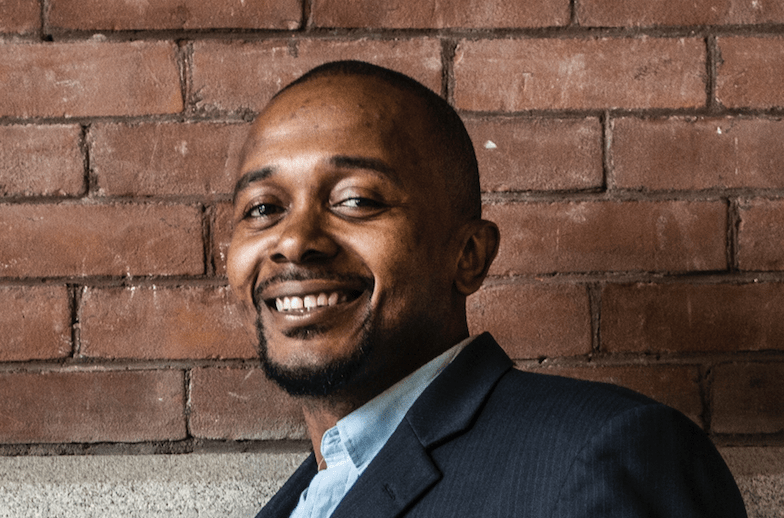
\includegraphics[width=0.13\textwidth]{images/Brandon-Ogbunu.png}
 \end{center}
\end{wrapfigure}
~\\ As part of our unit on the evolution of protein sequences, we are going to explore the work of C. Brandon Ogbunugafor. C. Brandon Ogbunugafor's lab studies the intersection of evolutionary biology, genetics, and epidemiology. He uses experimental evolution, mathematical modeling, and computational biology to better understand the underlying causes and consequences of disease, across scales: from the biophysics of proteins involved in drug resistance to the social determinants driving epidemics at the population level. He is a Professor at Yale University.

Please read the following article by Prof. Ogbunugafor: 
\begin{enumerate}
\item \texttt{\href{https://www.genetics.org/content/genetics/214/4/749.full.pdf}{https://www.genetics.org/content/genetics/214/4/749.full.pdf}}
\end{enumerate}

Also listen to the following short radio segment (you might wonder if this is the right podcast, since it doesn't immediately discuss science. It is the right podcast!):
\begin{enumerate}
\item \texttt{\href{https://soundcloud.com/sse-communications/c-brandon-ogbunu-story-collider-evolution-2019}{https://soundcloud.com/sse-communications/c-brandon-ogbunu-story-collider-evolution-2019}}
\end{enumerate}

\subsubsection*{Written Assignment} 
After reading C. Brandon Ogbunugafor's paper and listening to his podcast, write a reflection (max one page) on what you discovered. You might wish to address some of the following: 

\begin{enumerate}
\item What was most interesting to you in reviewing these resources?
\item What did you learn from these resources the evolution of proteins?
\item What new questions do you have after reviewing these resources?
\item What do these resources tell you about the types of people that do computational biology, or their motivations?
\end{enumerate}

\EndAccSupp{}
\end{document}
